\begin{figure*}[t]
    \centering
    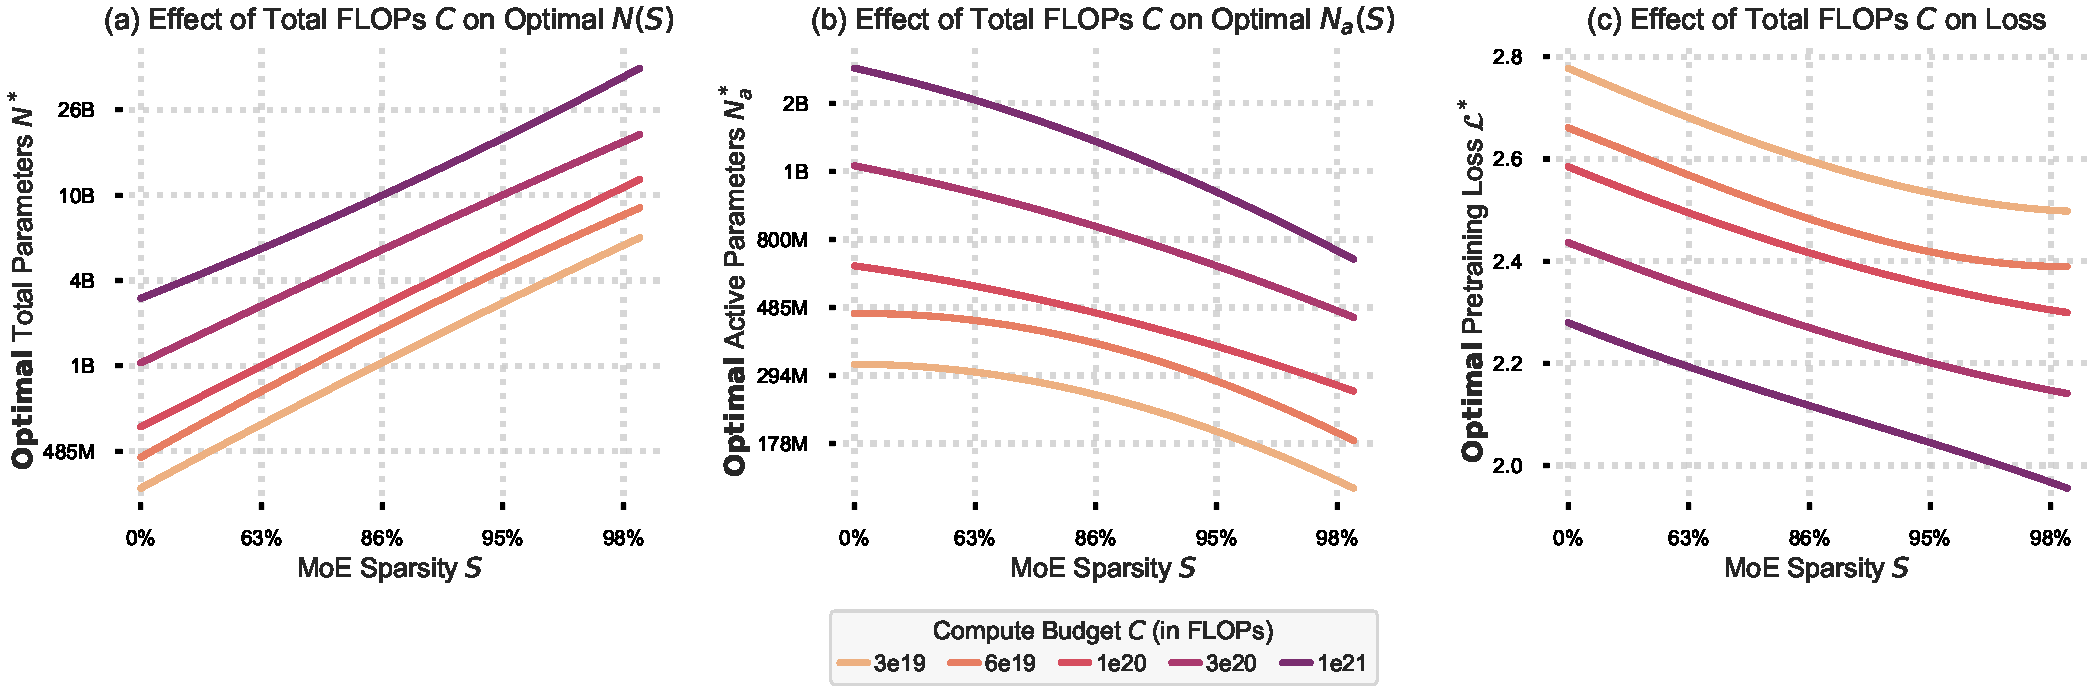
\includegraphics[width=0.8\textwidth]{plots/effect_of_total_flops_on_optimals.pdf}
    \caption{
    \textbf{Effect of compute budget on model size, number of active parameters and loss with sparsity.} Across all compute budgets, we observe that (a) the optimal model size $N$ increases with sparsity, (b) the optimal number of active parameters $N_a$ decreases with sparsity, and (c) the loss $L$ decreases with sparsity. 
    % We can see that larger models get sparser and have better performance at 
    % . (a) depict how optimal \( N \) increase with sparsity with a similar slope across different training compute budgets. (b) shows how optimal \( N_a\) decreases with sparsity across different sparsity levels. (c) shows how the loss for the compute optimal model decreases with sparsity across different compute budgets.
    % \Harshay{reminder to update plot if we decide to remove 1e21}
    }
    \label{fig:effect_of_compute}
    \vspace{-0.3cm}
\end{figure*}


\section{Impact of Training Compute Budget on the Interaction between Model Parameters and Sparsity} 
\label{sec:effect_of_training_budget}

Does increasing compute budget impact the interaction between the parameters and \flops per example in \moes and how they contribute to model's capacity?
In other words, does the recipe for optimally increasing model capacity, i.e., optimal sparsity level for \moes change as we scale up the total training compute? 

To answer this question. in \Cref{fig:effect_of_compute} we illustrate the trends for changing the total number of parameters, $N^*$, the number of active parameters, $N_a^*$, and the loss, $L^*$, with sparsity level across different compute budgets. 

\Cref{fig:effect_of_compute}c shows that the optimal sparsity level approaches 1 across all compute budgets used in our experiments. There is no significant difference observed in the slope of the loss vs sparsity curves across different training compute budgets used in our experiments. 
This observation suggests that there is no diminishing effect of sparsity on the pretraining loss as we increase training compute budget, i.e., if there is no constraint on the model size, sparsity improves the performance of the model across all training budgets.


In \Cref{fig:effect_of_compute}a and \Cref{fig:effect_of_compute}b, , we see a consistent trend of increasing \( N\) and decreasing \( N_a \) for compute optimal models as sparsity level increases across all training compute budgets.
Moreover, as can be seen in \Cref{fig:opt_sparsity}, when model size in terms of total number of parameters is fixed,  optimal sparsity level decreases with training compute budget while increases with model size as discussed in \Cref{sec:fix_params_vary_sparsity}.

\ifthenelse{\boolean{@twocolumn}}{
\begin{figure}
    \centering
    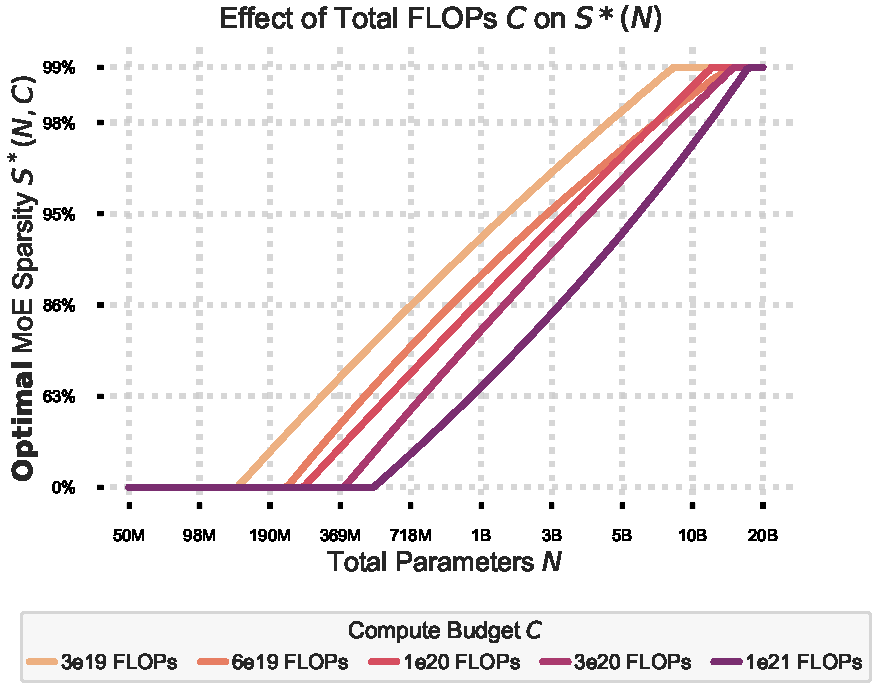
\includegraphics[width=0.45\textwidth]{plots/optimal_sparsity.pdf}
    \caption{\textbf{Effect of training budget $C$ and total parameters $N$ on MoE sparsity.} Optimal MoE sparsity $S^*$ changes with respect to the total number of parameters $N$ and the training budget $C$. The $x$-axis represents the total parameters $N$ on a logarithmic scale, and the $y$-axis shows the optimal MoE sparsity $S^*$.}
    \label{fig:opt_sparsity}
\end{figure}
}
{
\begin{wrapfigure}{r}{0.5\textwidth}
    \centering
    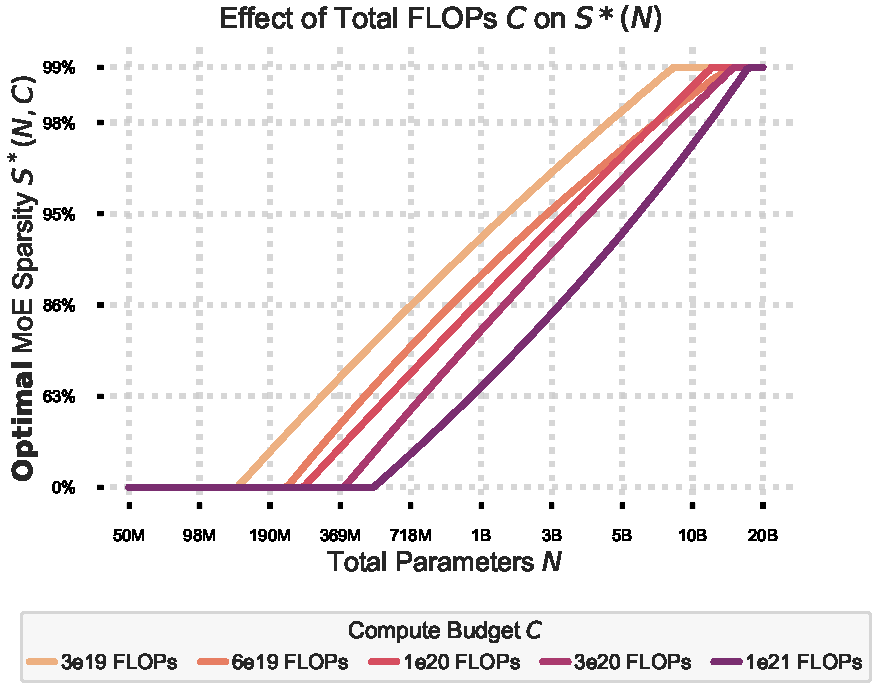
\includegraphics[width=0.45\textwidth]{plots/optimal_sparsity.pdf}
    \caption{\textbf{Effect of training budget $C$ and total parameters $N$ on MoE sparsity.} Optimal MoE sparsity $S^*$ changes with respect to the total number of parameters $N$ and the training budget $C$. The $x$-axis represents the total parameters $N$ on a logarithmic scale, and the $y$-axis shows the optimal MoE sparsity $S^*$.}
    \label{fig:opt_sparsity}
\end{wrapfigure}}

%  However, the rate of decreasing \( N_a \), which can be interpreted as inference cost, increases as we increase training compute budget. This means, at larger training compute budgets, the benefit of reducing compute in terms of FLOPs per example amplifies. i.e., the gains of increasing sparsity level to reduce inference cost becomes more significant at larger training budgets. 


% As the compute budget increases, the optimal sparsity level decreases for a fixed model size, while the expected optimal model size increases—both in terms of total parameters and active parameters. 

